
\begin{document}
\renewcommand{\thefigure}{SI.\arabic{figure}}
\setcounter{figure}{0}

\section*{Supplementary Information}\label{sec:SI}

\addcontentsline{toc}{section}{Supplementary Information}
\addtocontents{toc}{\setcounter{tocdepth}{-10}}
\renewcommand{\thesubsection}{SI.\arabic{subsection}}
\setcounter{subsection}{0}

\subsection{Vectorized model and abundance dynamics in community simulation}

The consumer and resource dynamics in the simulation is calculated using the vectorized version of equations 1 \& 2 for computing efficiency: 

\begin{align*}
&\frac{d\mathbf{C}}{dt} = diag(\mathbf{C}) \circ ((1-l) \mathbf{U} \cdot \mathbf{S} - \mathbf{R})\\
&\frac{d\mathbf{S}}{dt} = \boldsymbol{\rho} - diag(\mathbf{S})\cdot \mathbf{U}^T \cdot \mathbf{C} + (\mathbf{U} \cdot diag(\mathbf{S}) \cdot \mathbf{l})^T \cdot \mathbf{C}
\end{align*}
In these equations, $\mathbf{C}$ and $\mathbf{S}$ are single row matrices of consumer and resource concentration at each time point. $\mathbf{U}$ is the N $\times$ M matrix of species uptake rate, $\mathbf{R}$ is the single row matrix of species respiration rate with the length of N. $\mathbf{l}$ is the M $\times$ M leakage matrix for M resources, and l is the set leakage fraction of resources. "$\circ$" denotes the element wise product of two matrices, "$\cdot$" represents matrix multiplication, and "T" is the transpose of matrix. $diag(\mathbf{C})$ is setting the consumer concentration at each time point onto the diagonal of N $\times$ N matix with the rest of the elements as 0. $diag(\mathbf{S})$ is setting the resource concentration at each time point onto the diagonal of M $\times$ M matix with the rest of the elements as 0, which notation makes the calculation equivalent to calculating row-wise products of $\mathbf{U}$ and $\mathbf{S}$. 

The plot below (Figure \ref{fig:example}) shows an example of the abundance dynamics of $N = 100$ species of heterotrophic bacterial consumers competing for $M = 50$ resource types at $T_{ref}$ ($T = 0$ \textdegree C). The figure is plotted with 1000 time steps (which is before the system reaches steady state), however it has already shown that a large number of species' biomass drop to extinction shortly after the simulation started, while none of the resources went extinct.

\begin{figure}[H]
    \centering
    \begin{tabular}{c@{}c@{}}
    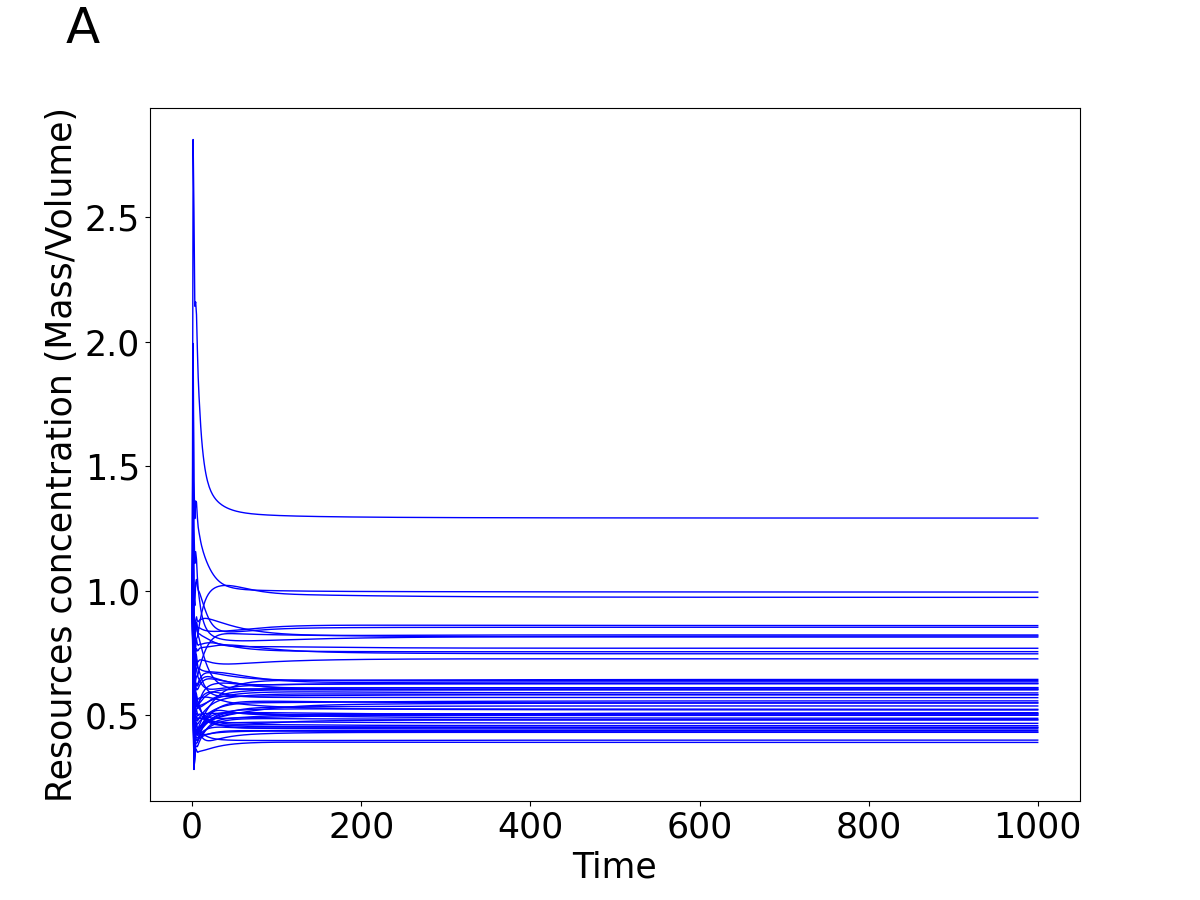
\includegraphics[scale=0.27]{./Figures/resource_con_example.png}
    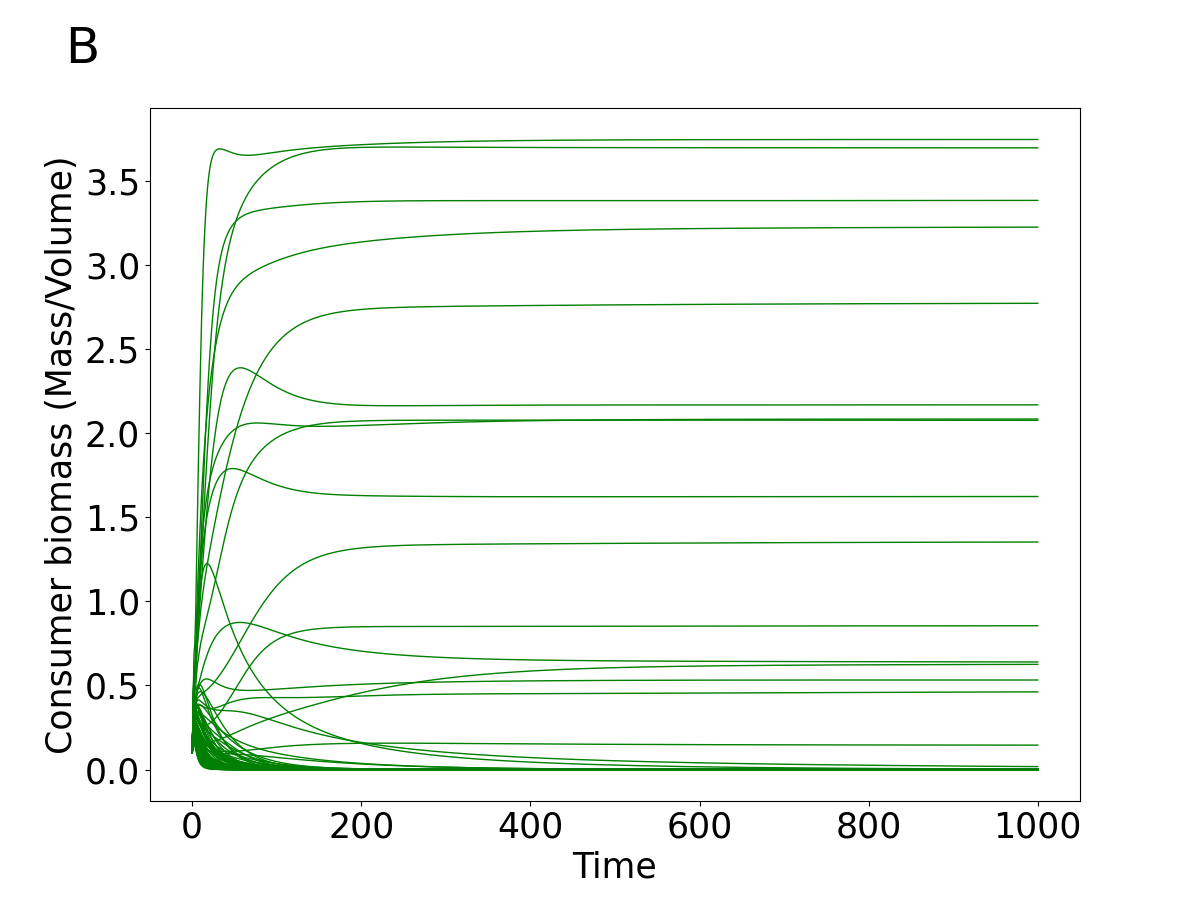
\includegraphics[scale=0.27]{./Figures/consumer_con_example.png}
    \end{tabular}
    \caption{\textbf{Example plots showing the resources concentration and consumers biomass dynamics of one assembly.} Plotted with 1000 time steps at reference temperature, $N = 100$ consumers competiting for $M = 50$ resources.}
    \label{fig:example}
\end{figure}

\subsection{TPCs of metabolic rates}

\begin{figure}[H]
    \centering
    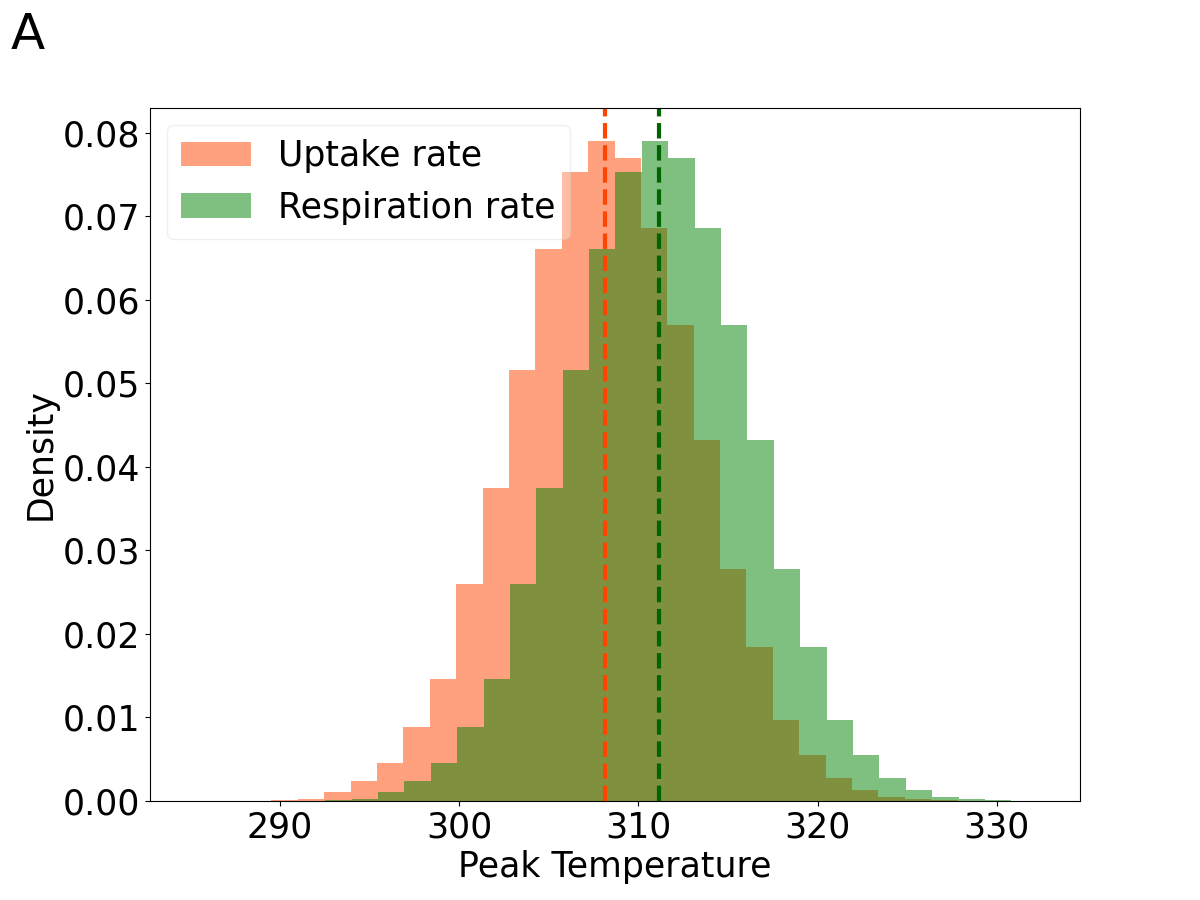
\includegraphics[scale=0.27]{./Figures/SI_UR.png}
    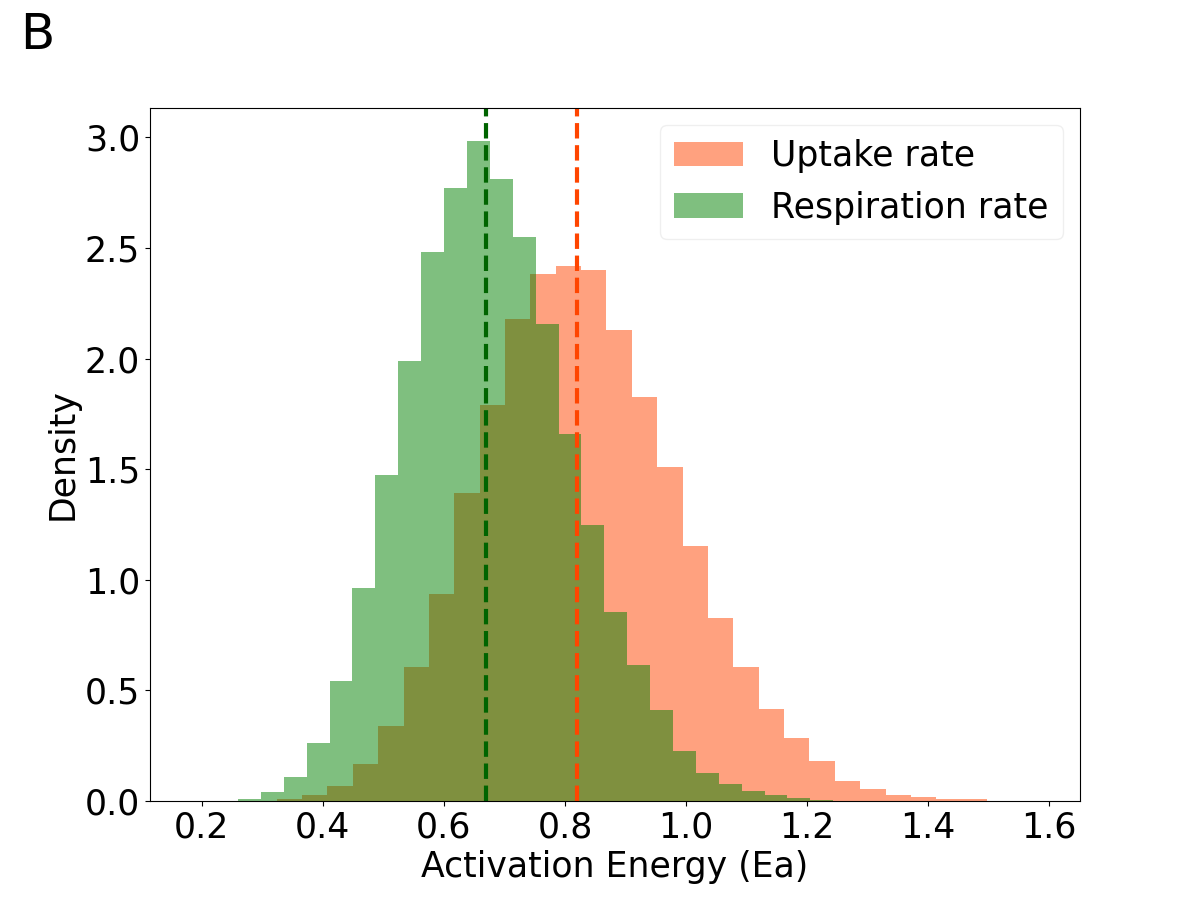
\includegraphics[scale=0.27]{./Figures/SI_UR_1.png}
    \caption{\textbf{Histogram of randomly sampled $T_{pk}$ and $E_a$ values for uptake and respiration rates.} A: $T_{pk_U}$ was sampled from a normal distribution with mean value at 308.15 $K$, and $T_{pk_R} = T_{pk_U} + 3$ to make sure species respiration always peak higher than uptake. The dotted lines in the middle depict the mean values of uptake (orange) and respiration (green) rates peak temperatures. B: $E_a$ values are sampled from beta distributions ($\alpha = 15$) with median values of 0.82 $eV$ and 0.67 $eV$ for uptake and respiration.The dotted lines in the middle depict the median values of the thermal sensitivities of uptake (orange) and respiration (green) rates. The densities are shown with 50000 randomly generated values. }
    \label{fig:SI_UR}
\end{figure}

\begin{figure}[H]
    \centering
    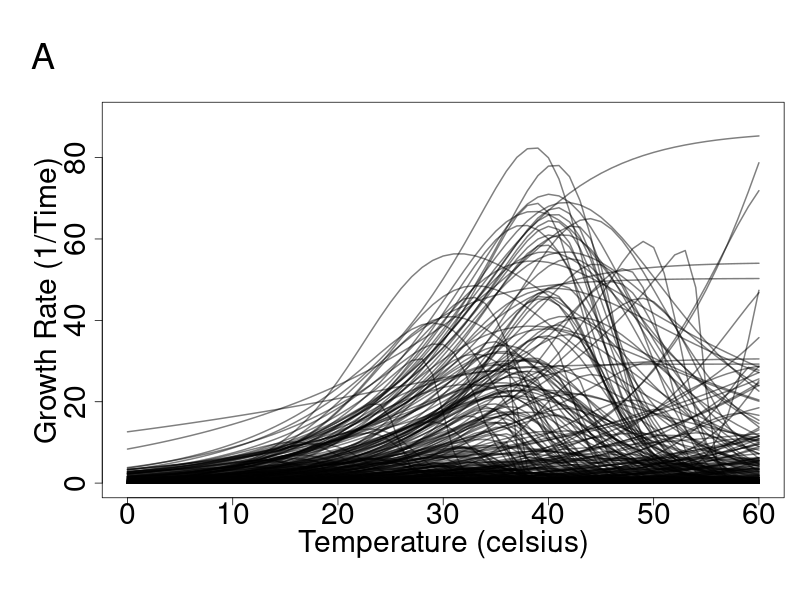
\includegraphics[scale=0.3]{./Figures/BioTrait_growth.png} \\
    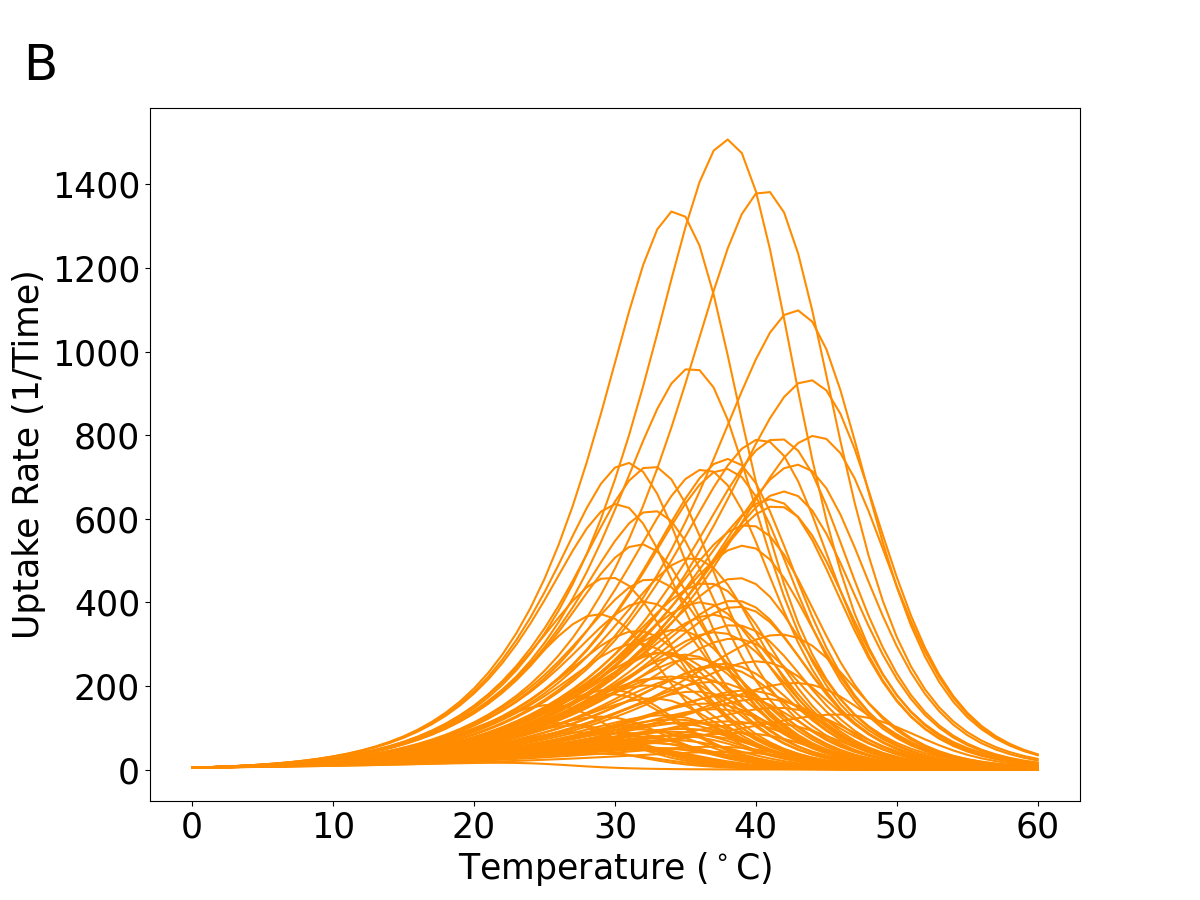
\includegraphics[scale=0.27]{./Figures/simulated_uptake_rate.png}
    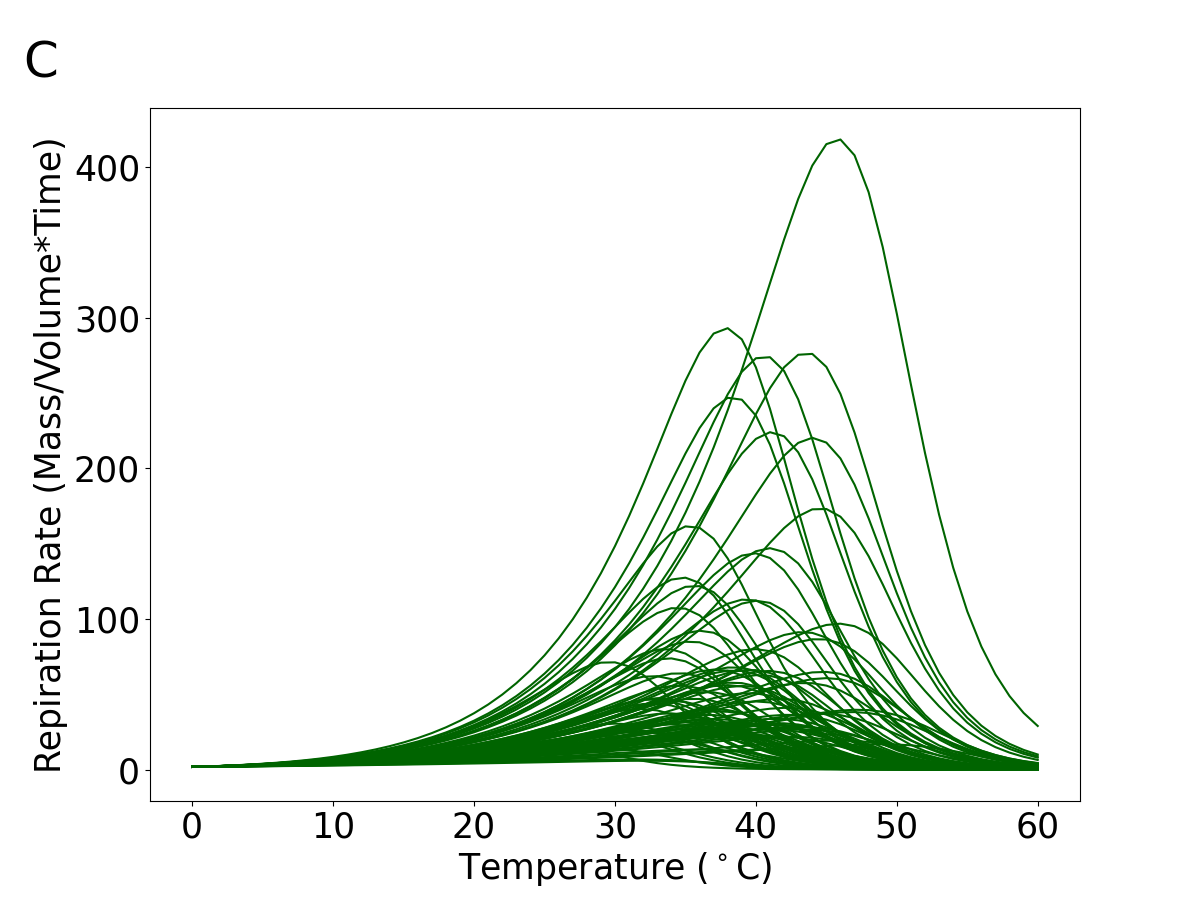
\includegraphics[scale=0.27]{./Figures/simulated_res_rate.png}
    \caption{\textbf{The temperature dependence curves of species growth, uptake and respiration rates.} A: The temperature performance curves of bacterial growth rates generated by fitting the modified Schoolfield temperature dependence equation, using the global data set collected and standardized by \cite{smith2019community}. B \& C: Example of a randomly generated set of temperature dependency curves for consumer uptake ($U_i$) and respiration ($R_i$) rates ($N$ = 100). Assuming resource uptake is majorly allocated to growth and respiration: $U \approx R + \mu$.}
    \label{fig:G}
\end{figure}

\subsection{Derivation of equations linking competitive exclusion and metabolic strategies}\label{sec:S+CUE}

The equilibrium resource concentration requirement for the $i^{th}$ species ($S^*$) can be calculated by rearranging equation \ref{eq:community} with $dC_i/dt = 0$, getting:

\begin{equation*}\label{eq:S*}
S^*_i = \frac{R_i}{U_i(1-l)}
\end{equation*}
The Arrhenius equation can be implanted here for species growing in OTR:

\begin{equation*}
S^*_i = \frac{R_0 e^{\frac{-Ea_R}{k}\cdot\left(\frac{1}{T} - \frac{1}{T_{ref}}\right)}}{U_0 e^{\frac{-Ea_U}{k}\cdot\left(\frac{1}{T} - \frac{1}{T_{ref}}\right)} (1-l)}
\end{equation*}
Take a log form of the equation, and set $\Delta T = \frac{1}{k}\left(\frac{1}{T} - \frac{1}{T_{ref}}\right) $:

\begin{equation*}
lnS^*_i = lnR_0 - ln(1-l)U_0 + (Ea_U - Ea_R) \Delta T
\end{equation*}

In this equation, since $R_0$ and $U_0$ values do not differ between species, the comparison of $S^*$ values lies completely in the differences between $Ea_U$ and $Ea_R$. Since at temperatures higher than reference temperature, the $\Delta T$ value is negative, so the species with higher $Ea_U - Ea_R$ value will have lower $S^*$, therefore winning the competition. 

In this case, the resource requirements for survival can be linked to species intrinsic CUE values (equation \ref{eq:CUE_i}), as:
\begin{equation}\label{eq:S_CUE}
CUE_i = (1 - S^*_i) (1-l)
\end{equation}
Therefore, the advantage of lower resource requirement in resource competition is related to the selection on higher intrinsic CUE values.

Since winner species with higher fitness (lower $S^*$) has higher $Ea_U - Ea_R$ value, these species also have higher $E_{a_{CUE}}$ (equation \ref{eq:EaCUE}). The relationship between species fitness and $E_{a_{CUE}}$ can also be shown in equation as:
\begin{equation}\label{eq:S_Ea}
lnS^*_i = lnR_0 - ln(1-l)U_0 + \frac{U_0(1-l) - R_0}{R_0}E_{a_{CUE}}\Delta T
\end{equation}

\begin{figure}[H]
    \centering
    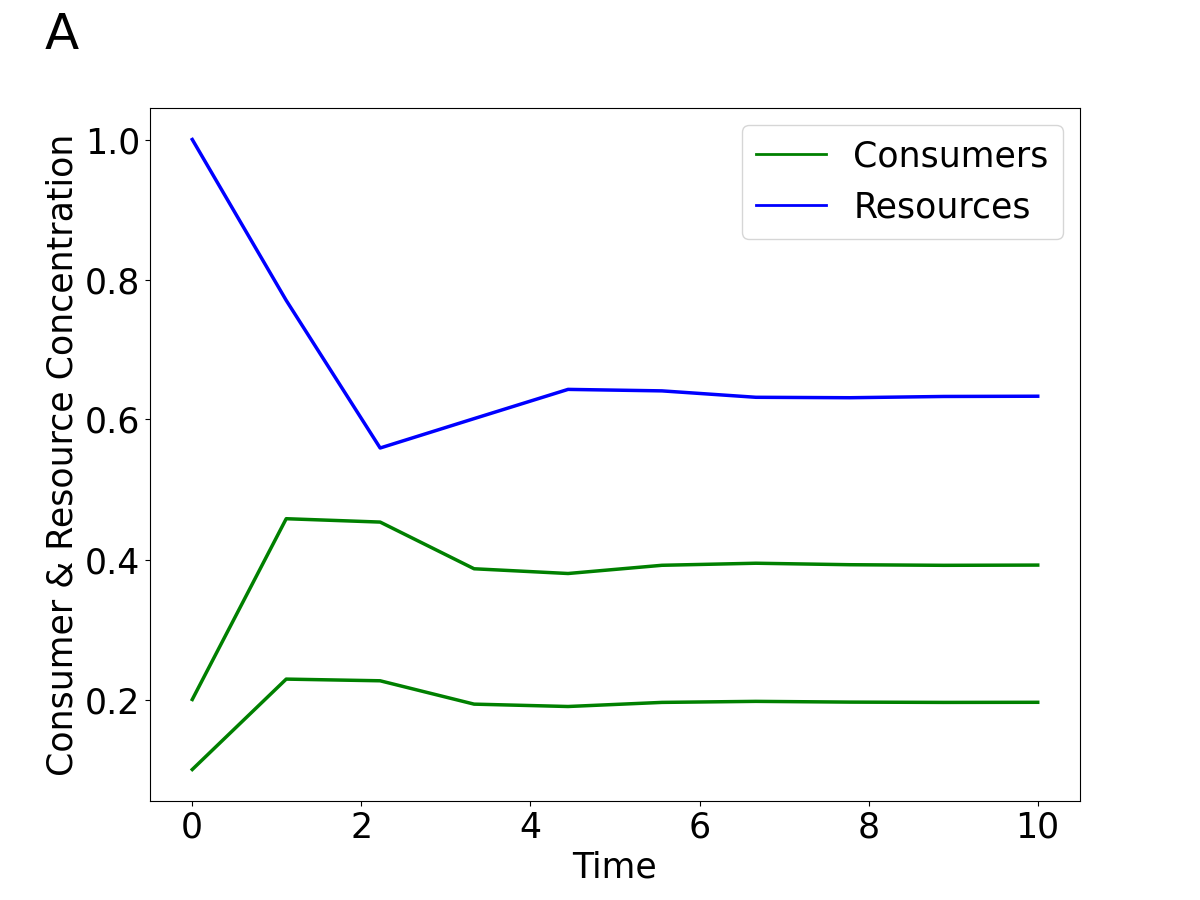
\includegraphics[scale=0.27]{./Figures/2_consumer_Tref.png}
    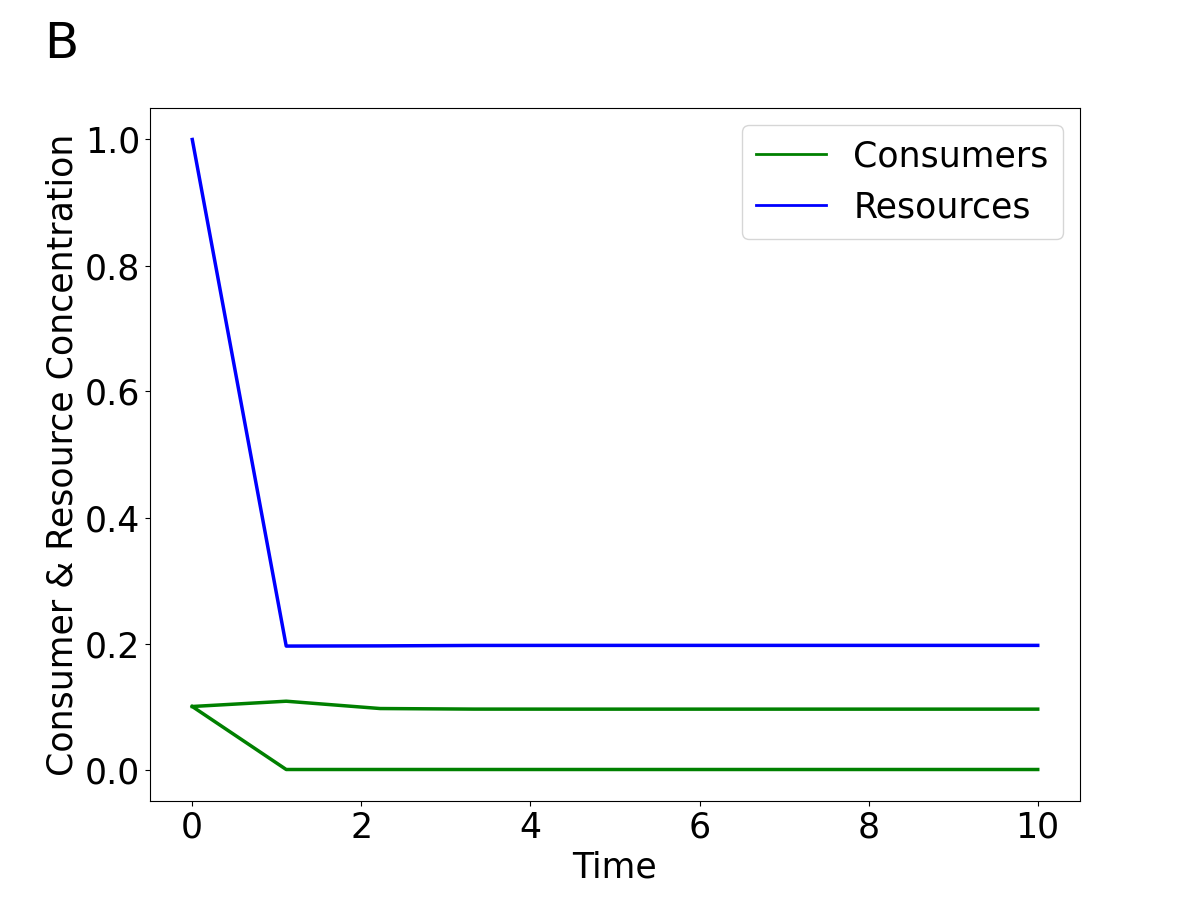
\includegraphics[scale=0.27]{./Figures/2_consumer_25C.png}
    \caption{\textbf{Example plots of the consumers and resource concentration dynamics of two species competing for one resource at reference temperature and at 25 \textdegree C.} A: At reference temperature, both species have the same $S^*$ therefore have the same growth rate regardless of their initial biomass. B: At temperatures higher than reference temperature, species have different $S^*$, competitive exclusion results in only one survivor.} 
    \label{fig:2_example}
\end{figure}

\subsection{Type II functional response}

For the robustness of qualitative results, I implemented Type II functional response (Monod function) into resources uptake. Note the resources uptake rates here has the unit of Mass/Volume*Time, which contains the concentration of species uptake at each time step. The uptake rate of $M^{th}$ resource by $i^{th}$ species: 
\begin{equation*}
    U_{m_{ij}} = U_{ij}\cdot\frac{S_j}{K+S_j}
\end{equation*}
K here is the half saturation constant of the $j^{th}$ resource. As shown in Figure \ref{fig:TypeII}B, implementing the Type II functional response into simulations does not significantly change the species richness pattern with assembly temperatures. 

\begin{figure}[H]
    \centering
    \begin{tabular}{c@{}c@{}}
    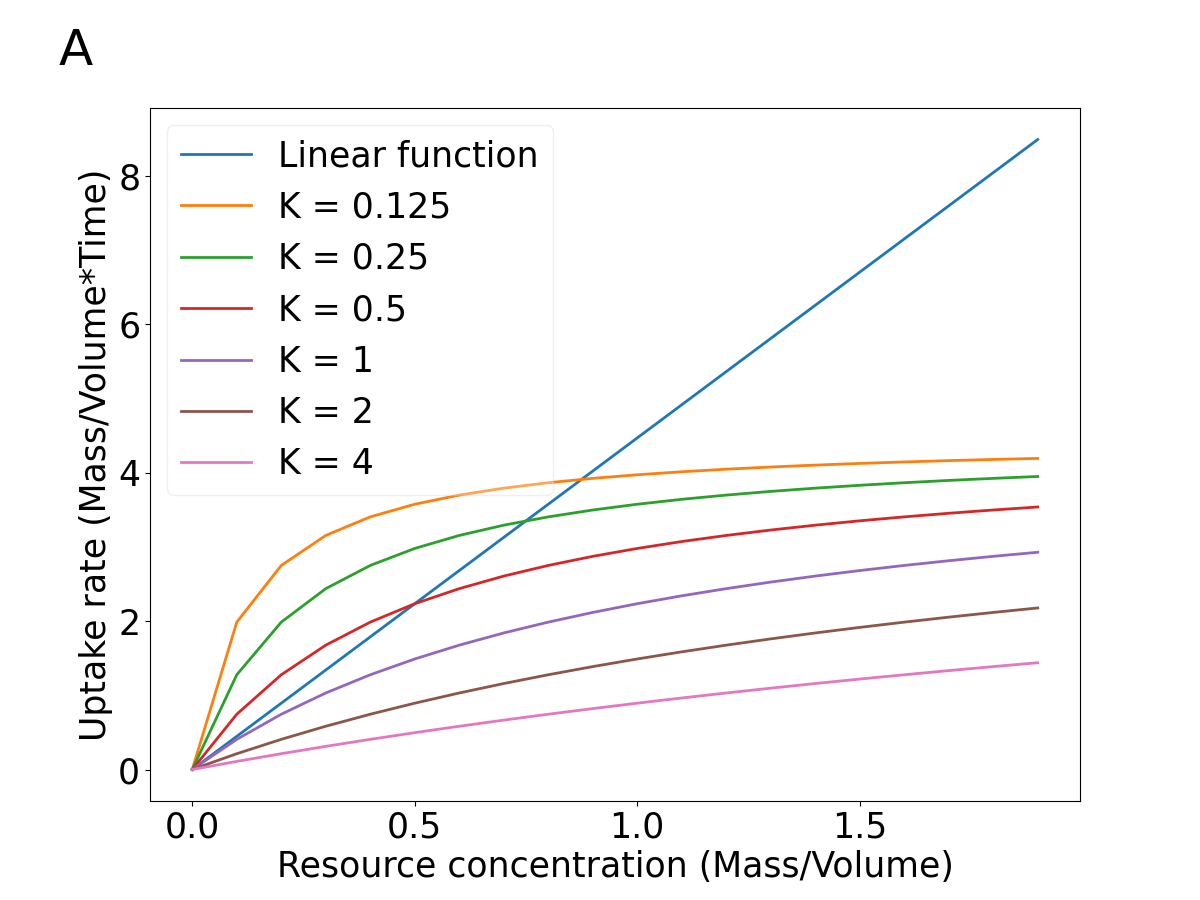
\includegraphics[scale=0.27]{./Figures/K.png}
    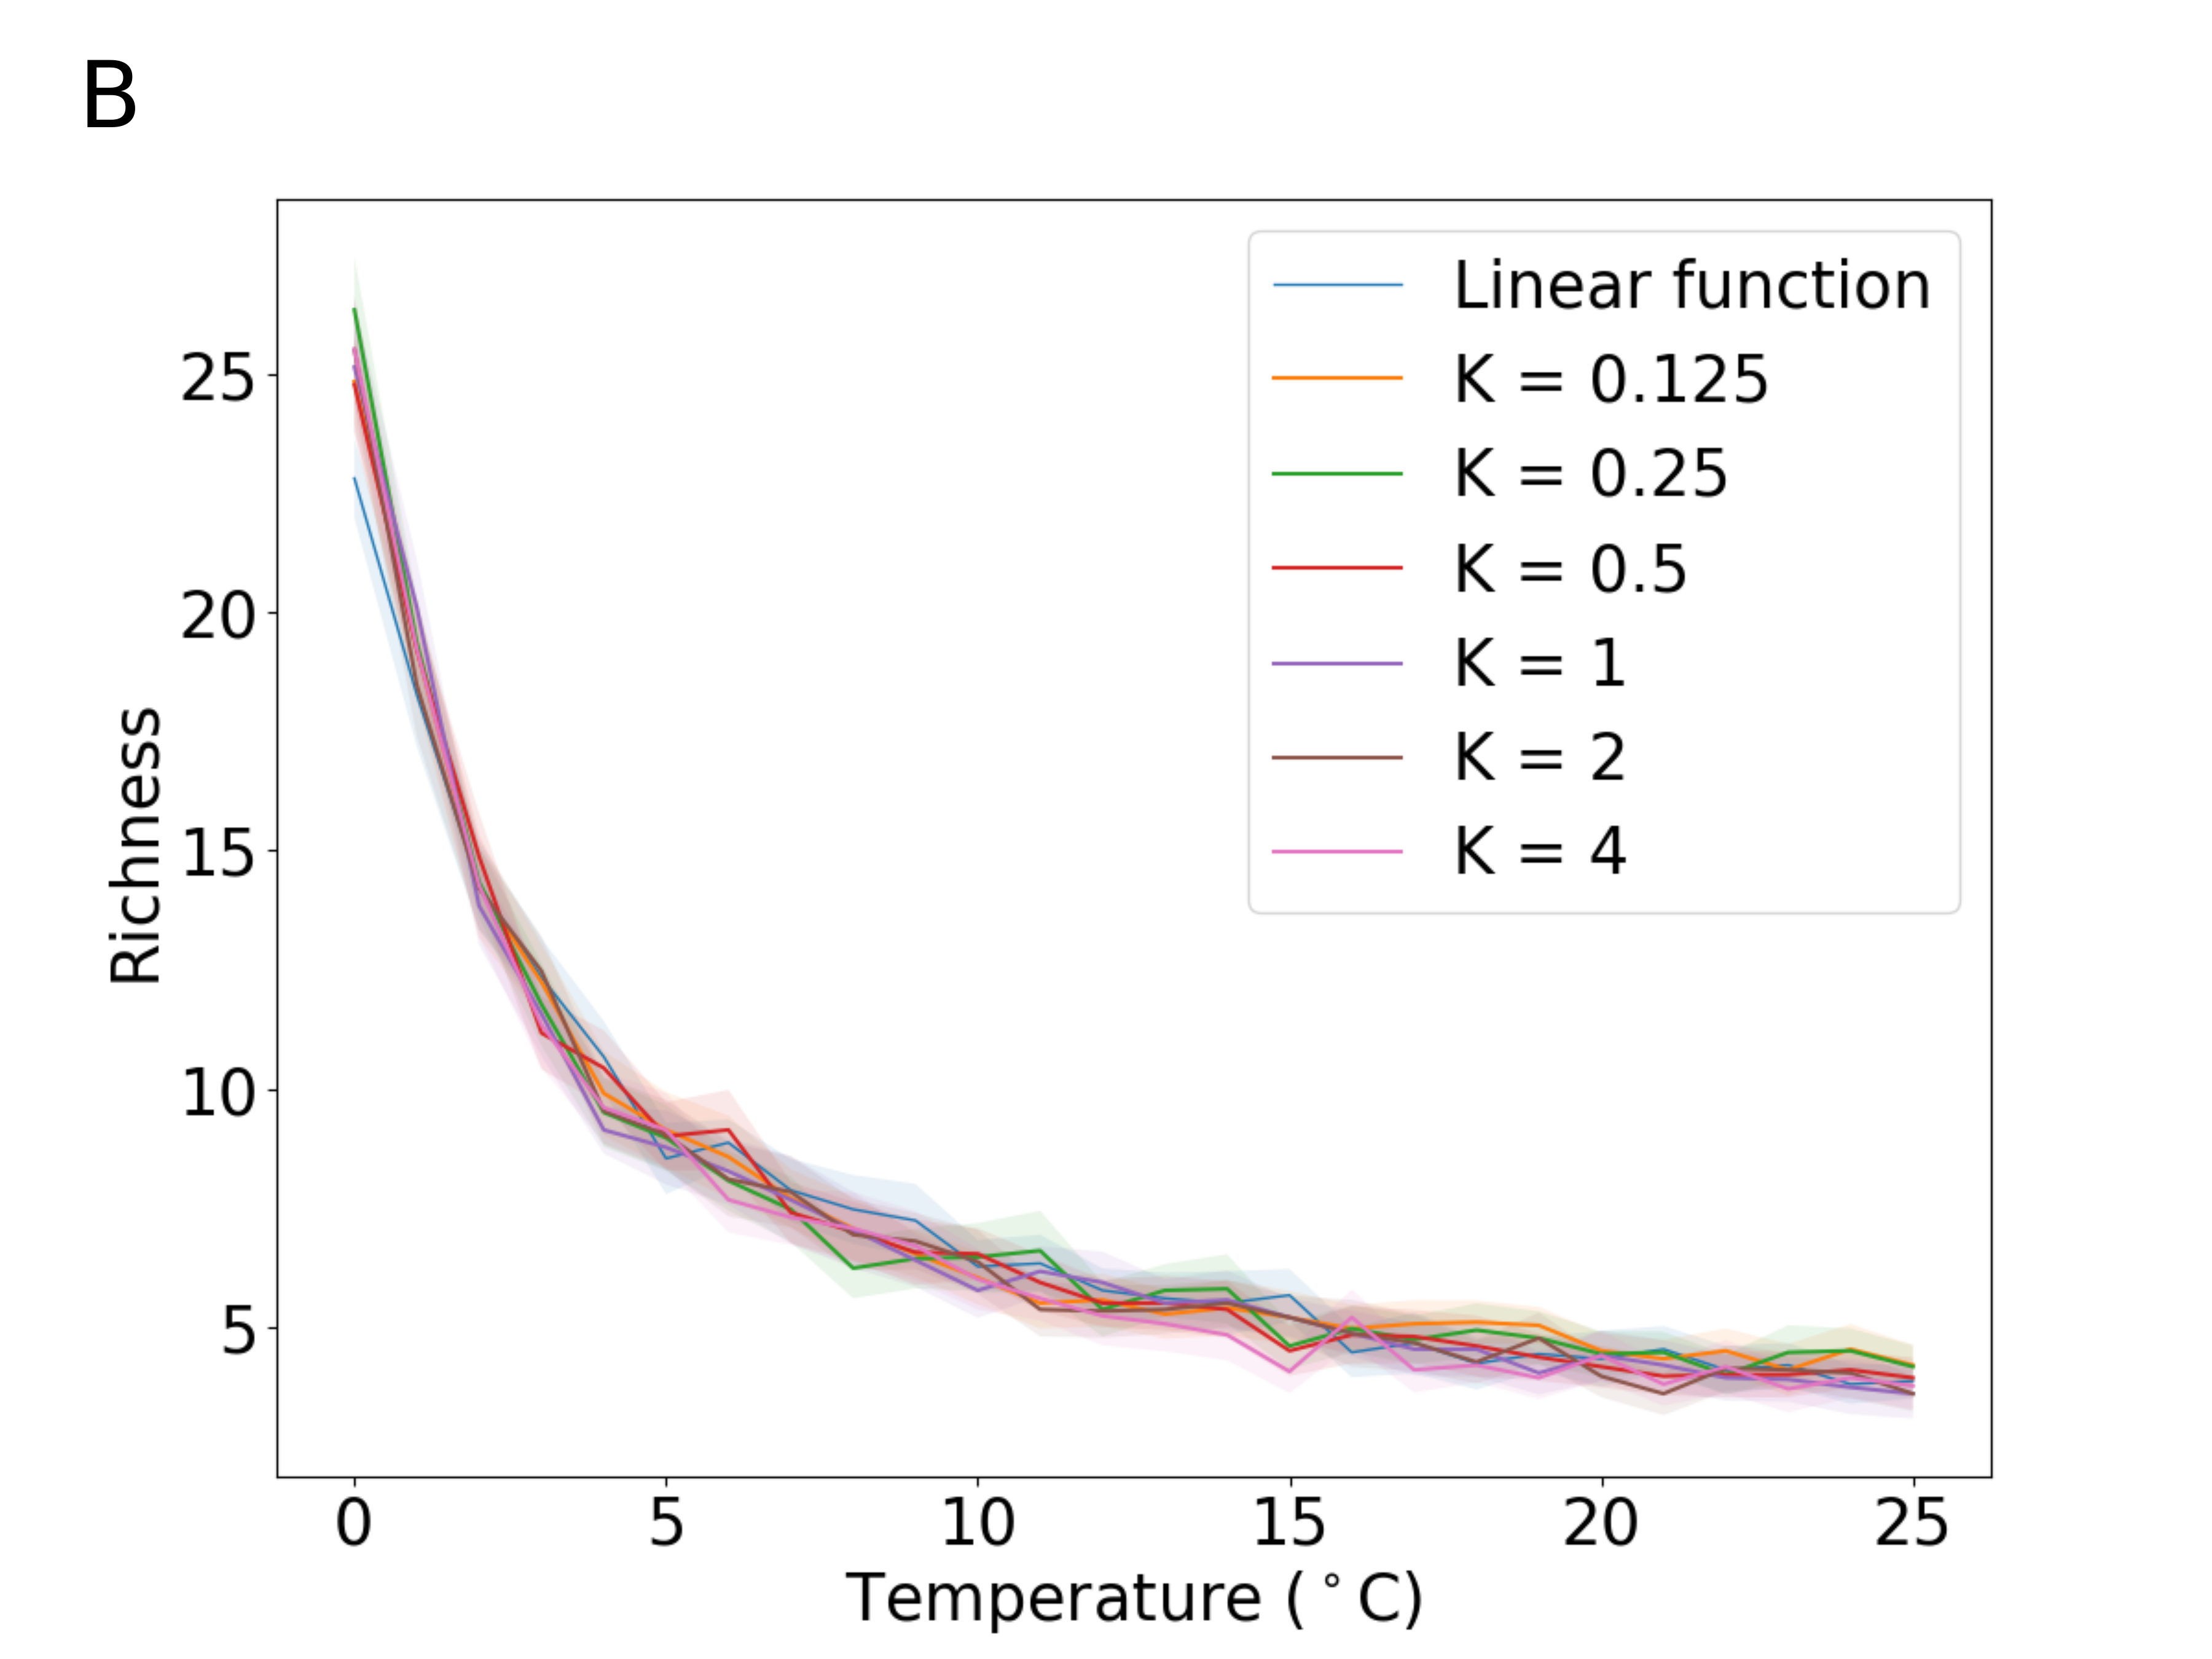
\includegraphics[scale=0.27]{./Figures/K_rich.png}
    \end{tabular}
    \hfill
    \begin{tabular}{c@{}c@{}}
    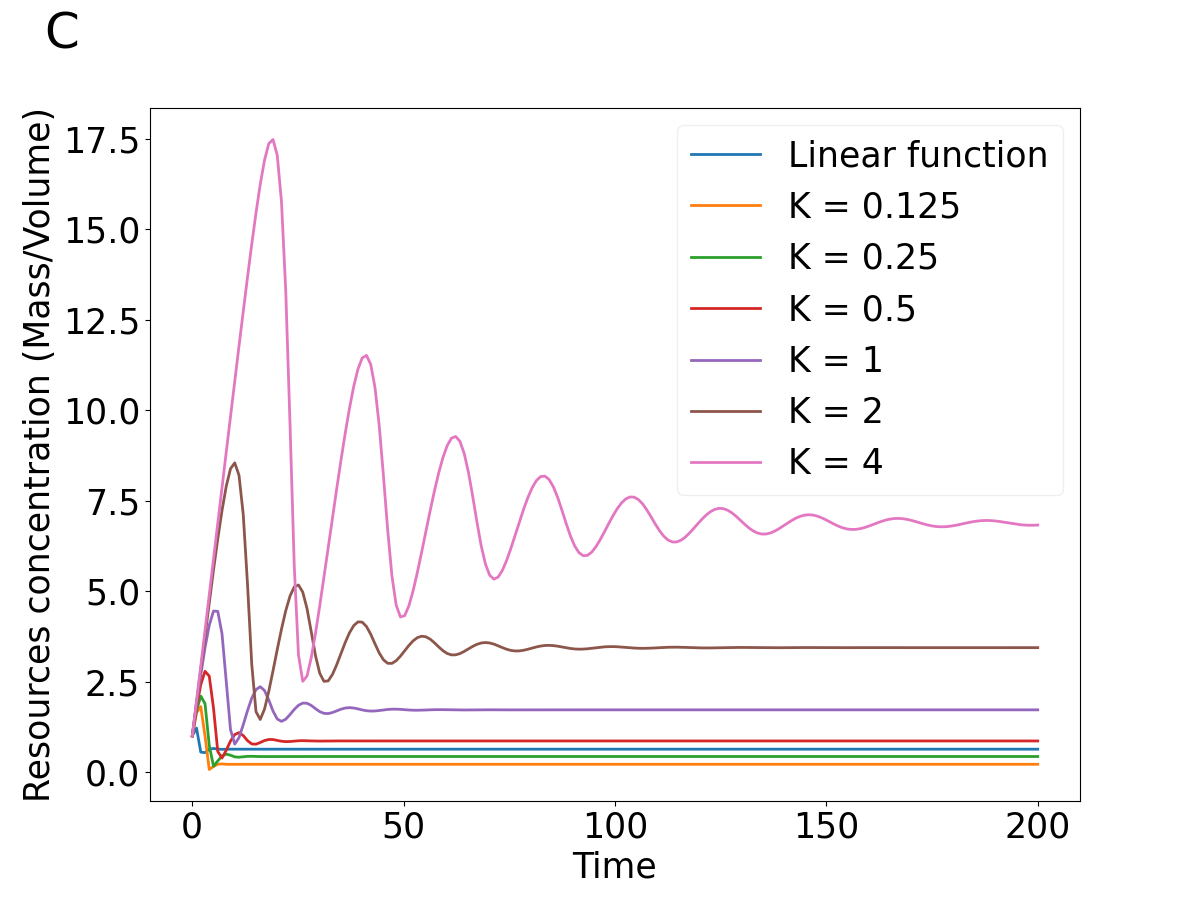
\includegraphics[scale=0.27]{./Figures/K_res.png}
    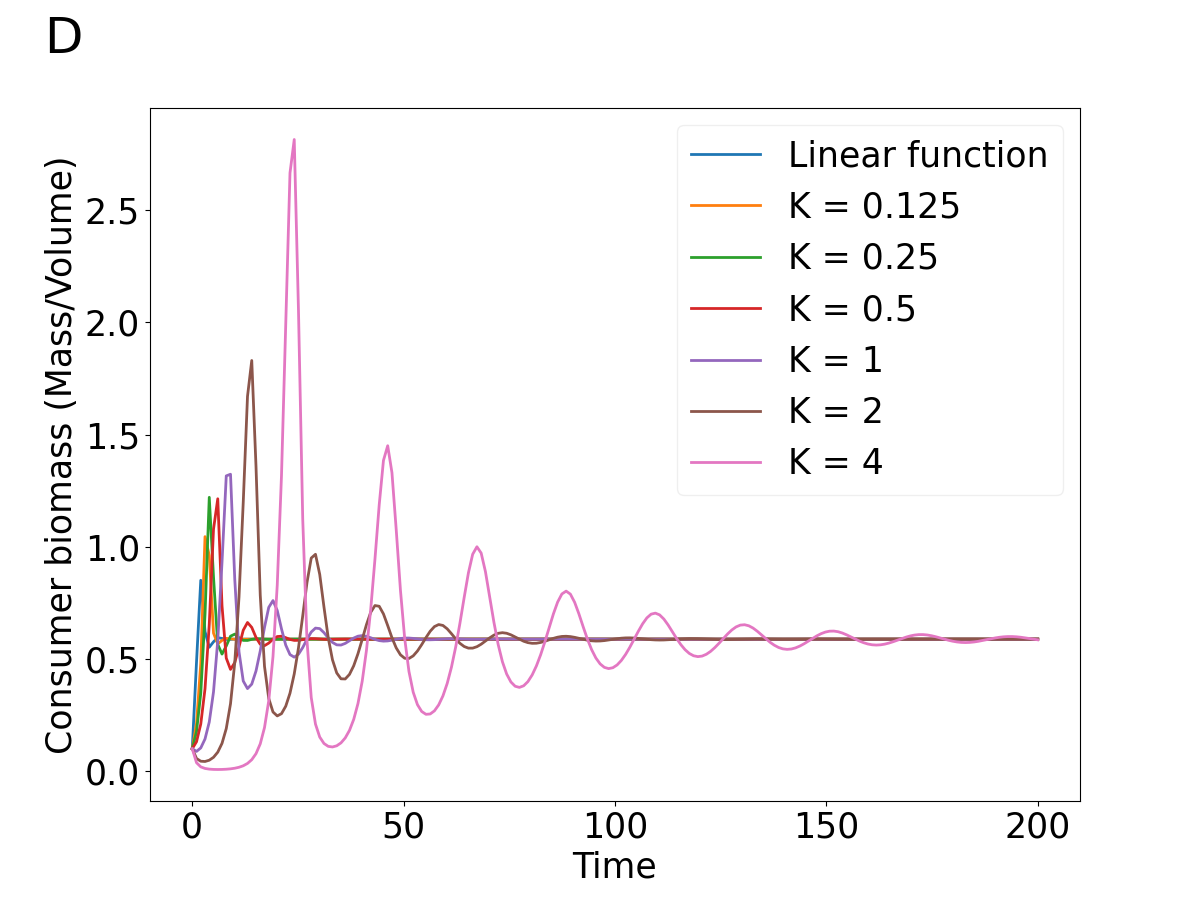
\includegraphics[scale=0.27]{./Figures/K_con.png}
    \end{tabular}
    \caption{\textbf{The temperature response of species richness with Type II functional response (Monod function) contained in species resource uptake.} A: The species uptake rates as a function of substrate resource concentration, $K$ denotes the half saturation constant. B: The temperature response of species richness with different K values. This plot shows that substituting linear functional response by Type II function response with different half saturation constants does not significantly impact species richness pattern with temperature. C \& D: The example of resource and consumer concentration dynamics of a single species with different half saturation constants in Monod function. }
    \label{fig:TypeII}
\end{figure}

\subsection{Interspeices interaction in high leakage environment}\label{sec:lf}

Here I show that changing leakage fractions does not significantly impact the temperature response pattern of species richness, with the exception of the highest leakage fraction of $l = 0.7$ (Figure \ref{fig:lf}A). And that that facilitation is favored at low temperatures for high leakage communities, at high temperatures for low leakage communities (Figure \ref{fig:lf}B). In Figure \ref{fig:lf}C, I demonstrate the interspecies interactions for communities with the extremely high leakage fraction of 0.7, it shows a sharper decrease of survivor resource overlap, and outweighing the increase of survivor facilitation at a lower temperature. Species with much higher resources partitions succeed competition (Figure \ref{fig:lf}D). Generally speaking, facilitation appears to be relatively unfavorable for communities at this leakage level. This indicates that facilitation is only beneficial for community coexistence to an extent, beyond that, the advantage of facilitative environment is outweighed by the detriments including the high resource leakage, and the extreme selection on species with lower resource overlap.

\begin{figure}
    \centering
    \begin{tabular}{c@{}c@{}}
    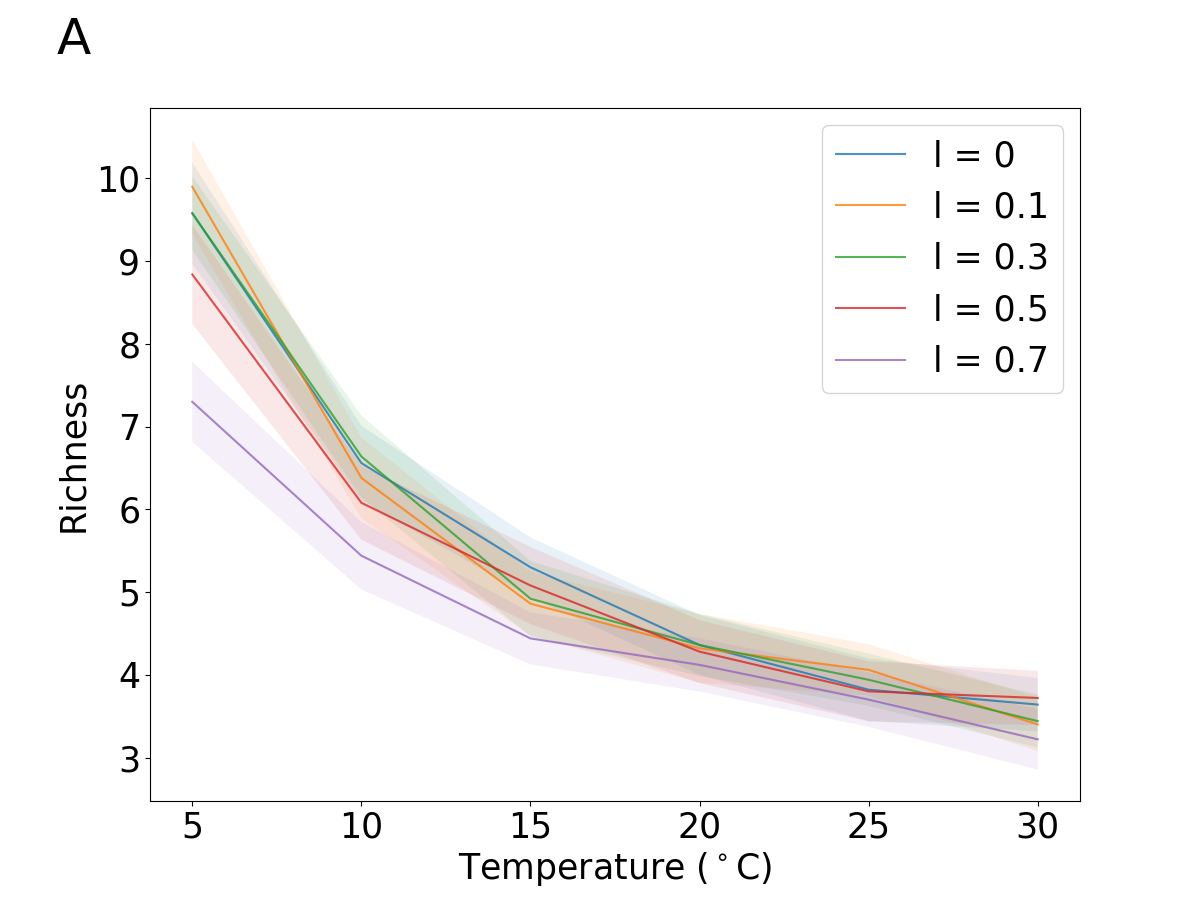
\includegraphics[scale=0.27]{./Figures/leakage_rich.png}
    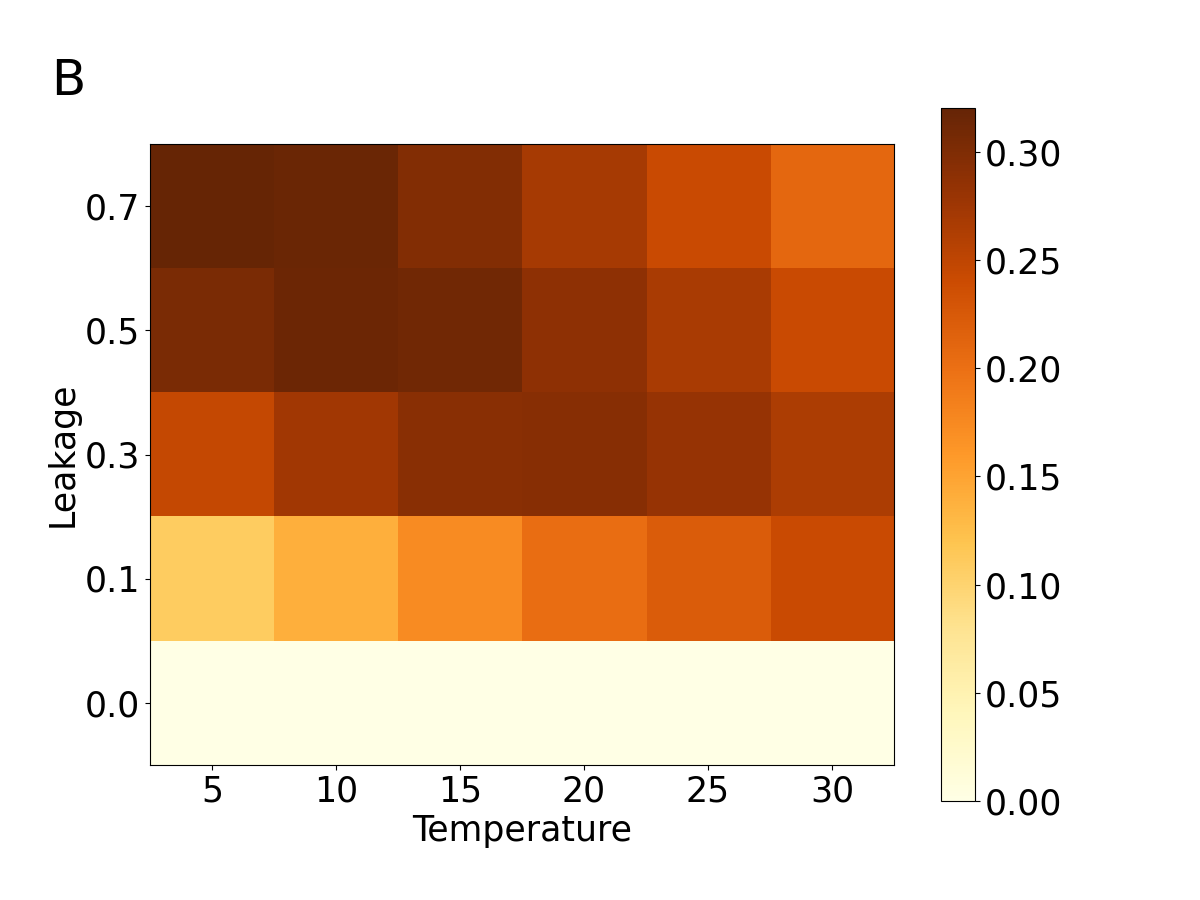
\includegraphics[scale=0.27]{./Figures/cf_lf.png}
    \end{tabular}
    \hfill\\
    \begin{tabular}{c@{}c@{}}
    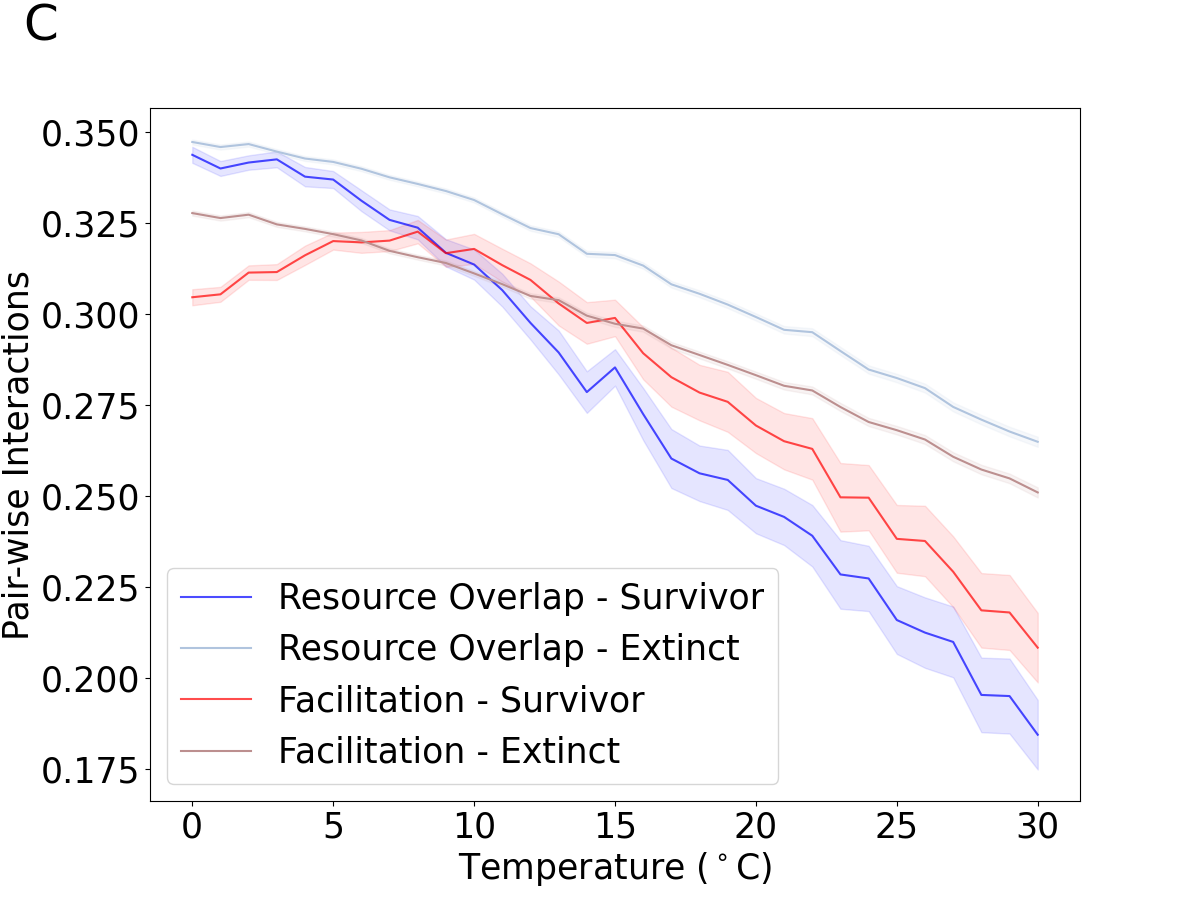
\includegraphics[scale=0.27]{./Figures/07.png}
    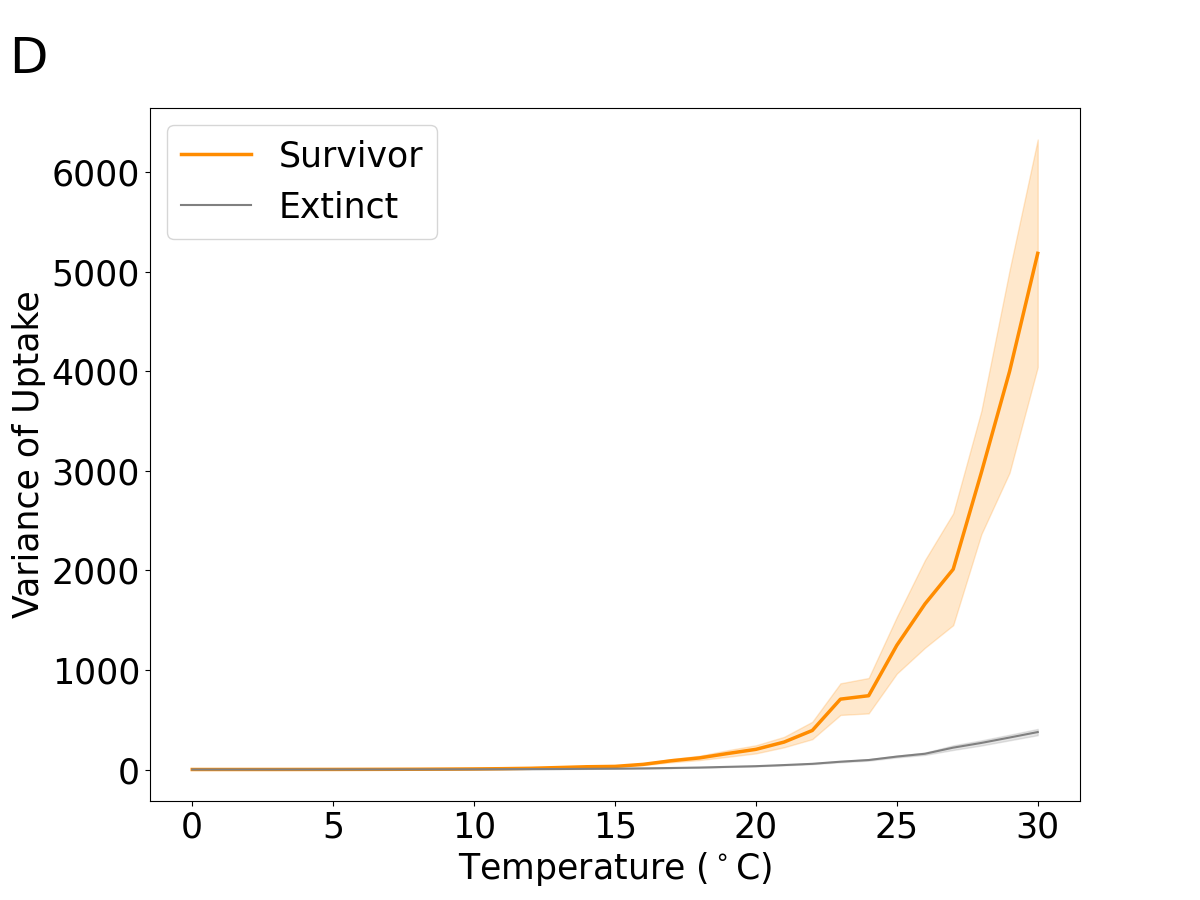
\includegraphics[scale=0.27]{./Figures/07_U.png}
    \end{tabular}
    \caption{\textbf{The relation between temperature dependent species richness pattern and the selection on interspecies facilitation.} Species richness at temperatures within OTR (A, plotted with 95\% CI bands for community richness values with each leakage fraction at each temperature) and the facilitation ability of survivors (B) at different leakage fraction and different temperatures. C and D demonstrates the resulting species interactions (C), and the variance of resources uptake (D) at different temperatures when setting leakage fraction to 0.7, with 95\% CI bands for these values in communities assembled at each temperature. (CI = 95\%)} 
    \label{fig:lf}
\end{figure}


\end{document}
